\section{影像翻译实验结果}

\subsection{数据准备}
\begin{frame}{当前章节}
    \tableofcontents[currentsection, currentsubsection]
\end{frame}

\begin{frame}{数据准备}
    数据使用 Michael Schmitt 的 SEN1-2\_DATASET
    
    其中包含56万张相同区域SAR影像与光学影像对\\[0.5cm]

    根据区域相似性, 制作数据集 
    \begin{itemize}
        \item 1000对影作为训练集
        \item 50对影像作为验证集
        \item 100对影像作为测试集
    \end{itemize}
    
    对于非监督学习, 则将监督学习数据对打散
    
    
\end{frame}

\subsection{pix2pix实验结果}

\begin{frame}{当前章节}
    \tableofcontents[currentsection, currentsubsection]
\end{frame}

\begin{frame}{pix2pix 实验结果}
    \begin{figure}[!htbp]
        \centering
        \subfloat[]{\label{fig:0101a}
        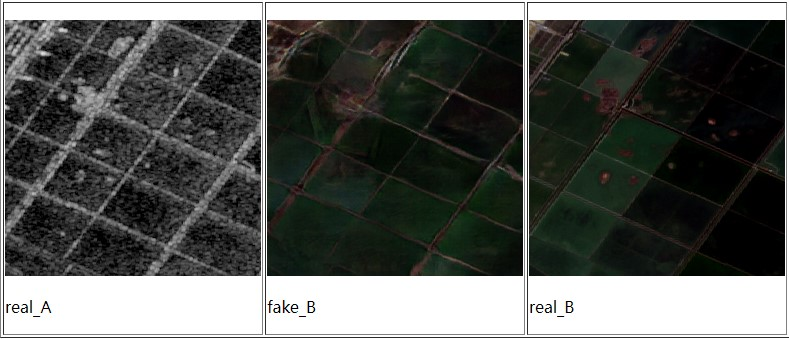
\includegraphics[height=2cm]{pic/chap0102.jpg}}
        \\[0.5cm]
        \subfloat[]{\label{fig:0101b}
        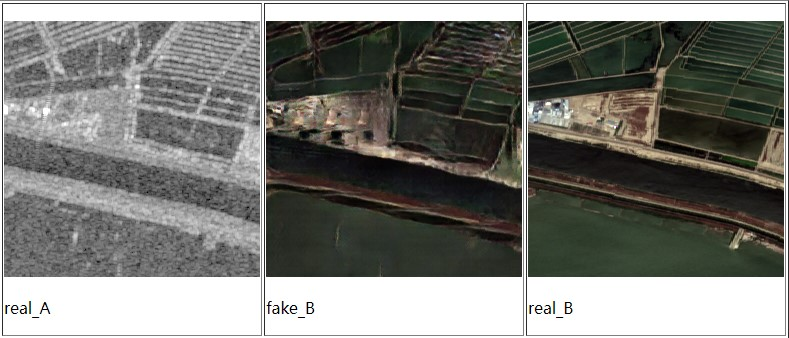
\includegraphics[height=2cm]{pic/chap0103.jpg}}
        \label{fig:0101}
        \caption{pix2pix 结果}
    \end{figure}  
\end{frame}

\begin{frame}{pix2pix 实验结果}
    \begin{figure}[!htbp]
        \centering
        \subfloat[]{\label{fig:0102a}
        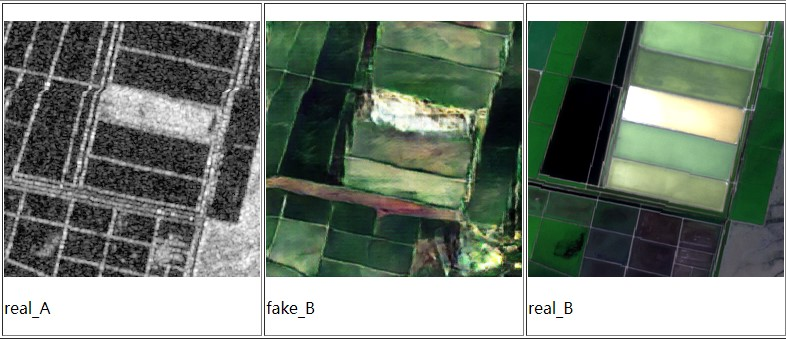
\includegraphics[height=2cm]{pic/chap0101.jpg}}
        \\[0.5cm]
        \subfloat[]{\label{fig:0102b}
        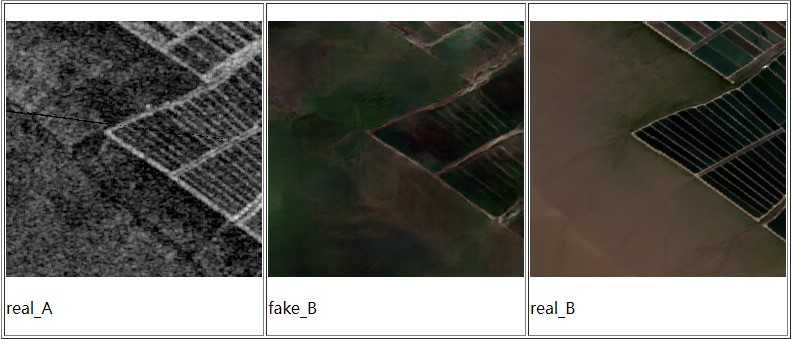
\includegraphics[height=2cm]{pic/chap0104.jpg}}
        \label{fig:0102}
        \caption{pix2pix 结果}
    \end{figure}  
\end{frame}

\subsection{cycleGAN实验结果}

\begin{frame}{当前章节}
    \tableofcontents[currentsection, currentsubsection]
\end{frame}

\begin{frame}{cycleGAN 实验结果}
    \begin{figure}[!htbp]
        \centering
        \subfloat[]{\label{fig:0103a}
        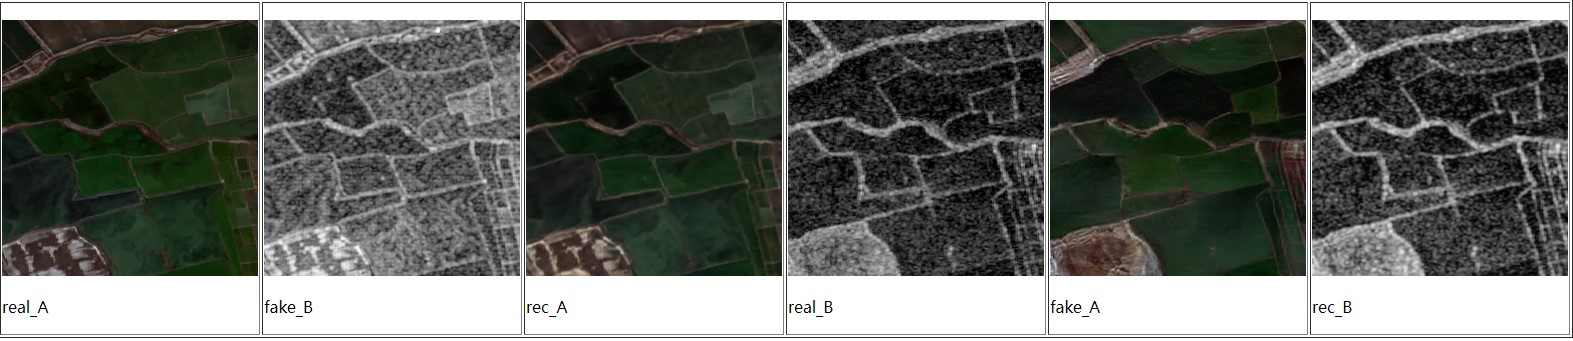
\includegraphics[height=2cm]{pic/chap0106.jpg}}
        \\[0.5cm]
        \subfloat[]{\label{fig:0103b}
        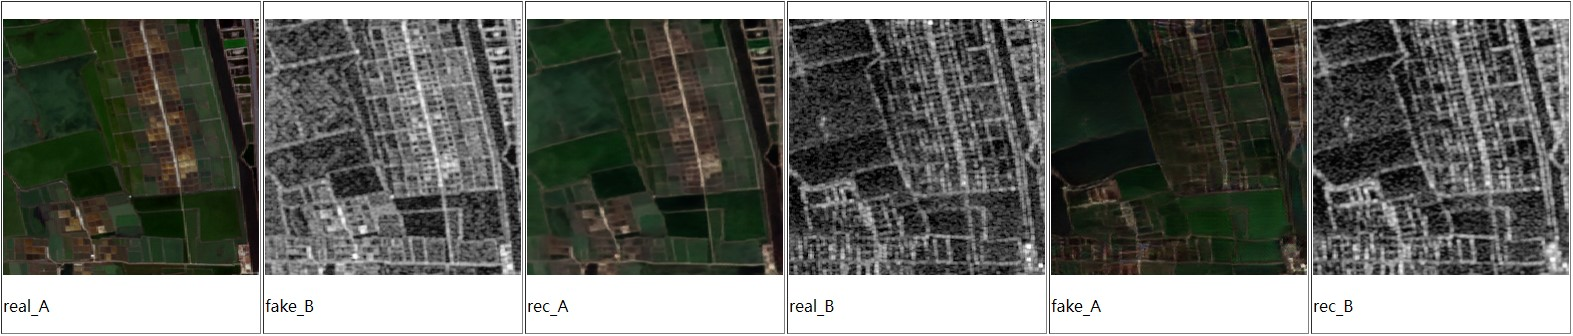
\includegraphics[height=2cm]{pic/chap0107.jpg}}
        \label{fig:0102}
        \caption{cycleGAN结果}
    \end{figure}  
\end{frame}

\begin{frame}{cycleGAN 实验结果}
    \begin{figure}[!htbp]
        \centering
        \subfloat[]{\label{fig:0104a}
        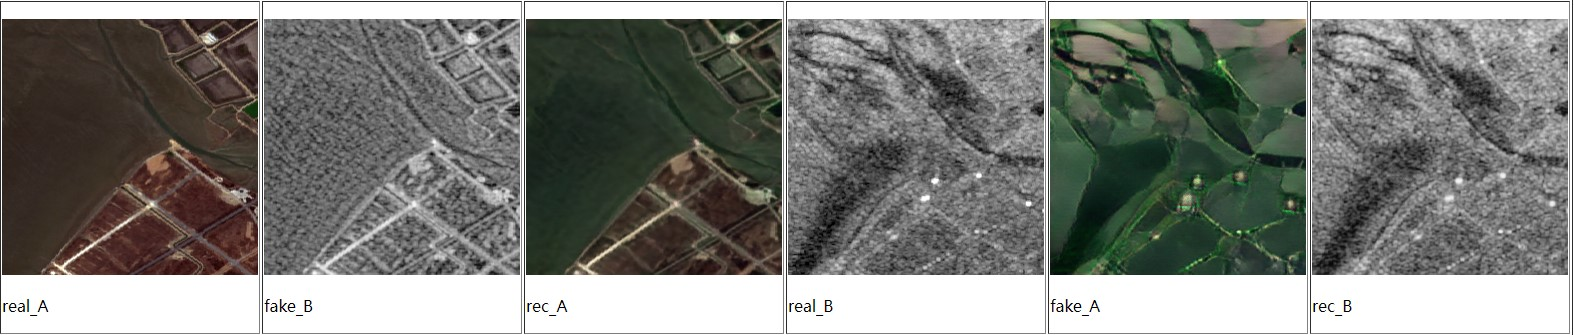
\includegraphics[height=2cm]{pic/chap0105.jpg}}
        \\[0.5cm]
        \subfloat[]{\label{fig:0104b}
        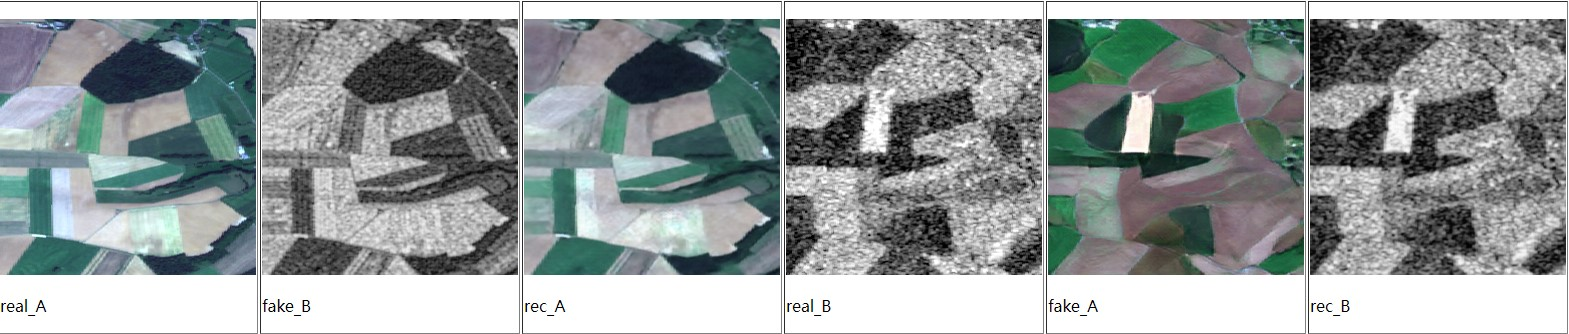
\includegraphics[height=2cm]{pic/chap0108.jpg}}
        \label{fig:0102}
        \caption{cycleGAN结果}
    \end{figure}  
\end{frame}

\subsection{结果分析}

\begin{frame}{当前章节}
    \tableofcontents[currentsection, currentsubsection]
\end{frame}

\begin{frame}{结果分析}
    存在问题有:
    \begin{itemize}
        \item 单维度到多维度的图像生成不确定
        \item 如何提高非监督学习影像翻译稳定性
        \item 如何评价翻译质量(与目标任务有关)
    \end{itemize}

    本周实验计划:
    \begin{itemize}
        \item 自制华南区域saropt数据集
        \item 针对sar2opt图像翻译问题看论文
    \end{itemize}
\end{frame}